\section{Paso 1: Introducción de datos}

  \paragraph{}Lo primero, y completamente necesario, para completar este
  ejemplo práctico, es crear toda la información que se necesita manejar, por
  parte del usuario \textit{Administrador principal}. Para ello, este usuario
  debe acceder a la aplicación con el nombre de usuario y contraseña con el que
  fue creado, como se vio en el capítulo \ref{instalacion},
  \textit{Instalación}. La figura \ref{capturaPaginaInicial} muestra la página
  inicial de la aplicación donde se debe realizar este acceso.

  \paragraph{}Una vez el usuario ha accedido a la zona del administrador
  principal, se procede a ingresar toda la información necesaria en el sistema.

  \subsection{Centro}

  \paragraph{}\textbf{Definición:} Se refiere al objeto del mundo real:
  \emph{``Institución académica de la Universidad de Córdoba donde se imparten
  títulos universitarios''}.

\subsubsection{Listar}

  \paragraph{}Para mostrar esta lista, es necesario establecer el centro para
  el que mostrar las asignaturas disponibles. Para ello, habrá que elegir el
  centro en la lista desplegable que se muestra en la figura
  \ref{capturaPantallaSelectCentro}.

  \paragraph{}También será necesario elegir la titulación a la que pertenecen
  las asignaturas, por lo que se elegirá entre las opciones de una lista
  desplegable, siguiendo el mismo mecanismo que para seleccionar centro. Se
  puede ver una captura de la selección de titulación en la figura
  \ref{capturaPantallaSelectTitulacion}.

  \begin{figure}[!ht]
    \begin{center}
      \fbox{
      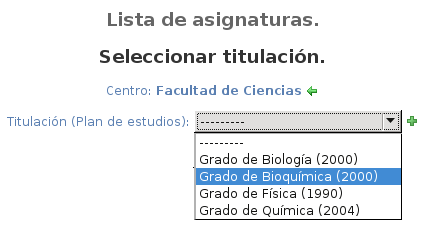
\includegraphics[scale=0.55]{4.Funcionamiento_Aplicacion/4.3.Gestion/4.3.1.Administrador_Principal/4.3.1.6.Asignatura/select_titulacion.png}
      }
      \caption{Captura de pantalla de la lista desplegable para seleccionar titulación para el usuario \textit{Administrador principal}.}
      \label{capturaPantallaSelectTitulacion}
    \end{center}
  \end{figure}

  \paragraph{}Nótese que si no existieran elementos disponibles en el sistema,
  la lista desplegable aparecería vacía. Por tanto, se proporciona al usuario
  un icono, representado por una cruz verde, para añadir nuevos elementos al
  sistema. Este icono es el mostrado en la figura \ref{capturaBotonAdd}. Al
  pulsar dicho botón, aparecerá la ventana de creación de un nuevo elemento.

  \paragraph{}Una vez seleccionados el centro y la titulación, se muestra la
  lista completa de asignaturas que aparecen en el sistema. La figura
  \ref{capturaPantallaListaAsignaturasAdminPrincipal} muestra
  una captura de pantalla de la lista de asignaturas.

  \begin{figure}[!ht]
    \begin{center}
      \fbox{
      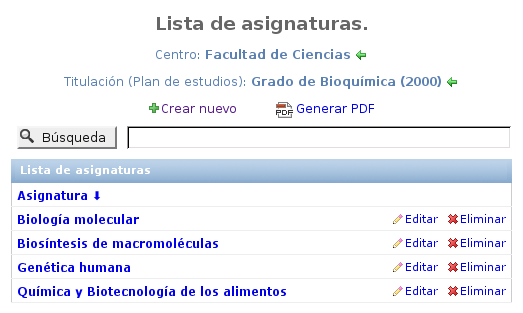
\includegraphics[scale=0.55]{4.Funcionamiento_Aplicacion/4.3.Gestion/4.3.1.Administrador_Principal/4.3.1.6.Asignatura/lista_asignaturas.png}
      }
      \caption{Captura de pantalla de la lista de asignaturas para el usuario \textit{Administrador principal}.}
      \label{capturaPantallaListaAsignaturasAdminPrincipal}
    \end{center}
  \end{figure}

  \paragraph{}Si se quisiera refinar el listado de elementos mostrados, es
  posible seleccionar nuevos parámetros pulsando el icono \textit{Seleccionar}
  que aparece al lado de cada elemento. Este icono aparece en la figura
  \ref{capturaBotonSeleccionar}.

\subsubsection{Añadir}

  \paragraph{}Para añadir un nuevo elemento al sistema, es necesario pulsar el
  icono \textit{Añadir nuevo}. Se puede ver una captura de pantalla de este
  icono en la figura \ref{capturaAddElemento}.

  \paragraph{}Al pulsar en el icono, se enlazará con el formulario de creación
  del nuevo elemento. Este formulario se puede ver en la imagen
  \ref{capturaAddReunionPreguntaAsesor}.

  \begin{figure}[!ht]
    \begin{center}
      \fbox{
      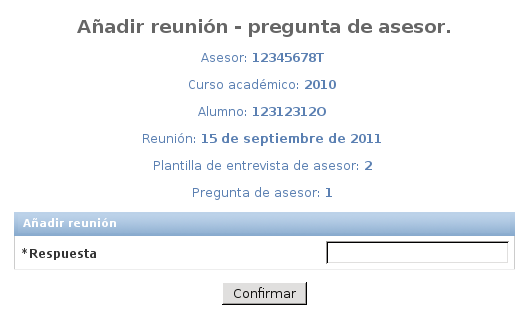
\includegraphics[scale=0.55]{4.Funcionamiento_Aplicacion/4.3.Gestion/4.3.1.Administrador_Principal/4.3.1.16.Reunion_PreguntaAsesor/add_reunion_preguntaAsesor.png}
      }
      \caption{Captura de pantalla del formulario para la creación de \textit{Reunión - Pregunta de asesor}.}
      \label{capturaAddReunionPreguntaAsesor}
    \end{center}
  \end{figure}

  \paragraph{}Una vez rellenado el formulario, se pulsará el botón
  \textit{Confirmar}, el cual se puede ver en la figura
  \ref{capturaBotonConfirmar}. Si el formulario rellenado es válido, y no tiene
  errores, se creará el nuevo elemento en el sistema. En caso de contener
  información no válida, un mensaje de error aparecerá indicando los campos
  del formulario que no han pasado la validación, los cuales habrá que modificar
  para introducir correctamente el elemento en el sistema.

\subsubsection{Editar}

  \paragraph{}Para editar un elemento del sistema, es necesario pulsar el
  icono \textit{Editar}. Se puede ver una captura de pantalla de este
  icono en la figura \ref{capturaEditElemento}. También es posible acceder
  al formulario de edición del elemento pulsando sobre el nombre del elemento
  que aparece en el listado.

  \paragraph{}Al pulsar en el icono, se enlazará con el formulario de edición
  del elemento. Este formulario se puede ver en la imagen
  \ref{capturaEditPreguntaOficial}.

  \begin{figure}[!ht]
    \begin{center}
      \fbox{
      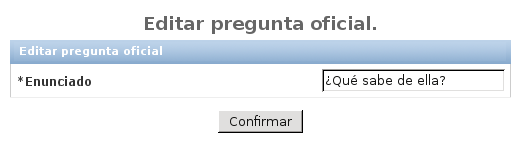
\includegraphics[scale=0.55]{4.Funcionamiento_Aplicacion/4.3.Gestion/4.3.1.Administrador_Principal/4.3.1.19.PreguntaOficial/edit_pregunta_oficial.png}
      }
      \caption{Captura de pantalla del formulario de edición de \textit{Pregunta oficial}.}
      \label{capturaEditPreguntaOficial}
    \end{center}
  \end{figure}

  \paragraph{}Una vez rellenado el formulario, se pulsará el botón
  \textit{Confirmar}, el cual se puede ver en la figura
  \ref{capturaBotonConfirmar}. Si el formulario rellenado es válido, y no tiene
  errores, se editará la información del elemento en el sistema. En caso de
  contener información no válida, un mensaje de error aparecerá indicando los
  campos del formulario que no han pasado la validación, los cuales habrá que
  modificar para modificar correctamente el elemento en el sistema.

  \subsection{Titulación}

  \paragraph{}\textbf{Definición}: Se refiere al objeto del mundo real:
  \emph{``Conjunto de materias cuya superación supone la obtención de un título
  académico''}.

\subsubsection{Listar}

  \paragraph{}Para mostrar esta lista, es necesario establecer el centro para
  el que mostrar las asignaturas disponibles. Para ello, habrá que elegir el
  centro en la lista desplegable que se muestra en la figura
  \ref{capturaPantallaSelectCentro}.

  \paragraph{}También será necesario elegir la titulación a la que pertenecen
  las asignaturas, por lo que se elegirá entre las opciones de una lista
  desplegable, siguiendo el mismo mecanismo que para seleccionar centro. Se
  puede ver una captura de la selección de titulación en la figura
  \ref{capturaPantallaSelectTitulacion}.

  \begin{figure}[!ht]
    \begin{center}
      \fbox{
      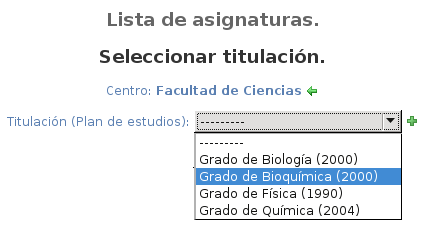
\includegraphics[scale=0.55]{4.Funcionamiento_Aplicacion/4.3.Gestion/4.3.1.Administrador_Principal/4.3.1.6.Asignatura/select_titulacion.png}
      }
      \caption{Captura de pantalla de la lista desplegable para seleccionar titulación para el usuario \textit{Administrador principal}.}
      \label{capturaPantallaSelectTitulacion}
    \end{center}
  \end{figure}

  \paragraph{}Nótese que si no existieran elementos disponibles en el sistema,
  la lista desplegable aparecería vacía. Por tanto, se proporciona al usuario
  un icono, representado por una cruz verde, para añadir nuevos elementos al
  sistema. Este icono es el mostrado en la figura \ref{capturaBotonAdd}. Al
  pulsar dicho botón, aparecerá la ventana de creación de un nuevo elemento.

  \paragraph{}Una vez seleccionados el centro y la titulación, se muestra la
  lista completa de asignaturas que aparecen en el sistema. La figura
  \ref{capturaPantallaListaAsignaturasAdminPrincipal} muestra
  una captura de pantalla de la lista de asignaturas.

  \begin{figure}[!ht]
    \begin{center}
      \fbox{
      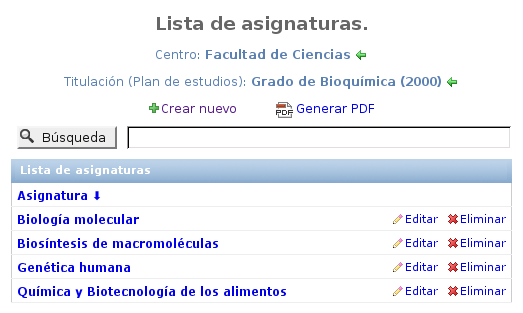
\includegraphics[scale=0.55]{4.Funcionamiento_Aplicacion/4.3.Gestion/4.3.1.Administrador_Principal/4.3.1.6.Asignatura/lista_asignaturas.png}
      }
      \caption{Captura de pantalla de la lista de asignaturas para el usuario \textit{Administrador principal}.}
      \label{capturaPantallaListaAsignaturasAdminPrincipal}
    \end{center}
  \end{figure}

  \paragraph{}Si se quisiera refinar el listado de elementos mostrados, es
  posible seleccionar nuevos parámetros pulsando el icono \textit{Seleccionar}
  que aparece al lado de cada elemento. Este icono aparece en la figura
  \ref{capturaBotonSeleccionar}.

\subsubsection{Añadir}

  \paragraph{}Para añadir un nuevo elemento al sistema, es necesario pulsar el
  icono \textit{Añadir nuevo}. Se puede ver una captura de pantalla de este
  icono en la figura \ref{capturaAddElemento}.

  \paragraph{}Al pulsar en el icono, se enlazará con el formulario de creación
  del nuevo elemento. Este formulario se puede ver en la imagen
  \ref{capturaAddReunionPreguntaAsesor}.

  \begin{figure}[!ht]
    \begin{center}
      \fbox{
      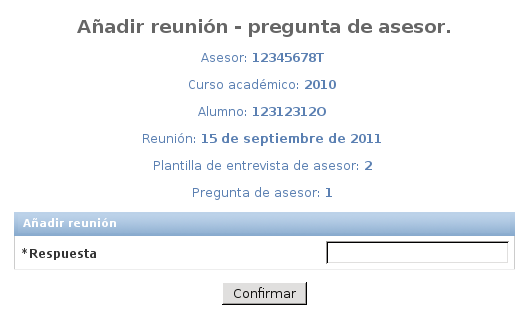
\includegraphics[scale=0.55]{4.Funcionamiento_Aplicacion/4.3.Gestion/4.3.1.Administrador_Principal/4.3.1.16.Reunion_PreguntaAsesor/add_reunion_preguntaAsesor.png}
      }
      \caption{Captura de pantalla del formulario para la creación de \textit{Reunión - Pregunta de asesor}.}
      \label{capturaAddReunionPreguntaAsesor}
    \end{center}
  \end{figure}

  \paragraph{}Una vez rellenado el formulario, se pulsará el botón
  \textit{Confirmar}, el cual se puede ver en la figura
  \ref{capturaBotonConfirmar}. Si el formulario rellenado es válido, y no tiene
  errores, se creará el nuevo elemento en el sistema. En caso de contener
  información no válida, un mensaje de error aparecerá indicando los campos
  del formulario que no han pasado la validación, los cuales habrá que modificar
  para introducir correctamente el elemento en el sistema.

\subsubsection{Editar}

  \paragraph{}Para editar un elemento del sistema, es necesario pulsar el
  icono \textit{Editar}. Se puede ver una captura de pantalla de este
  icono en la figura \ref{capturaEditElemento}. También es posible acceder
  al formulario de edición del elemento pulsando sobre el nombre del elemento
  que aparece en el listado.

  \paragraph{}Al pulsar en el icono, se enlazará con el formulario de edición
  del elemento. Este formulario se puede ver en la imagen
  \ref{capturaEditPreguntaOficial}.

  \begin{figure}[!ht]
    \begin{center}
      \fbox{
      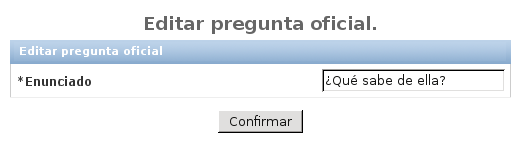
\includegraphics[scale=0.55]{4.Funcionamiento_Aplicacion/4.3.Gestion/4.3.1.Administrador_Principal/4.3.1.19.PreguntaOficial/edit_pregunta_oficial.png}
      }
      \caption{Captura de pantalla del formulario de edición de \textit{Pregunta oficial}.}
      \label{capturaEditPreguntaOficial}
    \end{center}
  \end{figure}

  \paragraph{}Una vez rellenado el formulario, se pulsará el botón
  \textit{Confirmar}, el cual se puede ver en la figura
  \ref{capturaBotonConfirmar}. Si el formulario rellenado es válido, y no tiene
  errores, se editará la información del elemento en el sistema. En caso de
  contener información no válida, un mensaje de error aparecerá indicando los
  campos del formulario que no han pasado la validación, los cuales habrá que
  modificar para modificar correctamente el elemento en el sistema.

  \subsection{Asignatura}\label{gestionAsignatura}

  \paragraph{}\textbf{Definición}: Se refiere al objeto del mundo real:
  \emph{``Materia que  forma parte del plan de estudios de una titulación''}.

\subsubsection{Listar}

  \paragraph{}Para mostrar esta lista, es necesario establecer el centro para
  el que mostrar las asignaturas disponibles. Para ello, habrá que elegir el
  centro en la lista desplegable que se muestra en la figura
  \ref{capturaPantallaSelectCentro}.

  \paragraph{}También será necesario elegir la titulación a la que pertenecen
  las asignaturas, por lo que se elegirá entre las opciones de una lista
  desplegable, siguiendo el mismo mecanismo que para seleccionar centro. Se
  puede ver una captura de la selección de titulación en la figura
  \ref{capturaPantallaSelectTitulacion}.

  \begin{figure}[!ht]
    \begin{center}
      \fbox{
      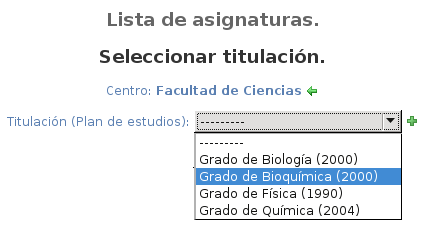
\includegraphics[scale=0.55]{4.Funcionamiento_Aplicacion/4.3.Gestion/4.3.1.Administrador_Principal/4.3.1.6.Asignatura/select_titulacion.png}
      }
      \caption{Captura de pantalla de la lista desplegable para seleccionar titulación para el usuario \textit{Administrador principal}.}
      \label{capturaPantallaSelectTitulacion}
    \end{center}
  \end{figure}

  \paragraph{}Nótese que si no existieran elementos disponibles en el sistema,
  la lista desplegable aparecería vacía. Por tanto, se proporciona al usuario
  un icono, representado por una cruz verde, para añadir nuevos elementos al
  sistema. Este icono es el mostrado en la figura \ref{capturaBotonAdd}. Al
  pulsar dicho botón, aparecerá la ventana de creación de un nuevo elemento.

  \paragraph{}Una vez seleccionados el centro y la titulación, se muestra la
  lista completa de asignaturas que aparecen en el sistema. La figura
  \ref{capturaPantallaListaAsignaturasAdminPrincipal} muestra
  una captura de pantalla de la lista de asignaturas.

  \begin{figure}[!ht]
    \begin{center}
      \fbox{
      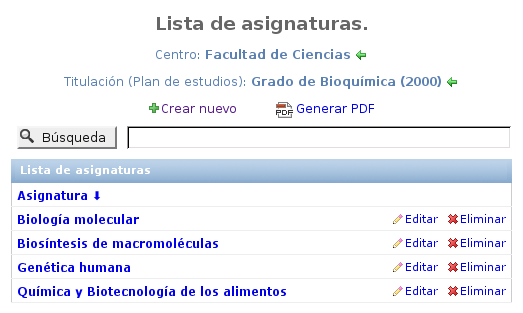
\includegraphics[scale=0.55]{4.Funcionamiento_Aplicacion/4.3.Gestion/4.3.1.Administrador_Principal/4.3.1.6.Asignatura/lista_asignaturas.png}
      }
      \caption{Captura de pantalla de la lista de asignaturas para el usuario \textit{Administrador principal}.}
      \label{capturaPantallaListaAsignaturasAdminPrincipal}
    \end{center}
  \end{figure}

  \paragraph{}Si se quisiera refinar el listado de elementos mostrados, es
  posible seleccionar nuevos parámetros pulsando el icono \textit{Seleccionar}
  que aparece al lado de cada elemento. Este icono aparece en la figura
  \ref{capturaBotonSeleccionar}.

\subsubsection{Añadir}

  \paragraph{}Para añadir un nuevo elemento al sistema, es necesario pulsar el
  icono \textit{Añadir nuevo}. Se puede ver una captura de pantalla de este
  icono en la figura \ref{capturaAddElemento}.

  \paragraph{}Al pulsar en el icono, se enlazará con el formulario de creación
  del nuevo elemento. Este formulario se puede ver en la imagen
  \ref{capturaAddReunionPreguntaAsesor}.

  \begin{figure}[!ht]
    \begin{center}
      \fbox{
      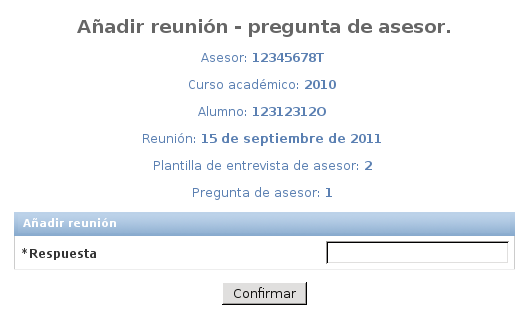
\includegraphics[scale=0.55]{4.Funcionamiento_Aplicacion/4.3.Gestion/4.3.1.Administrador_Principal/4.3.1.16.Reunion_PreguntaAsesor/add_reunion_preguntaAsesor.png}
      }
      \caption{Captura de pantalla del formulario para la creación de \textit{Reunión - Pregunta de asesor}.}
      \label{capturaAddReunionPreguntaAsesor}
    \end{center}
  \end{figure}

  \paragraph{}Una vez rellenado el formulario, se pulsará el botón
  \textit{Confirmar}, el cual se puede ver en la figura
  \ref{capturaBotonConfirmar}. Si el formulario rellenado es válido, y no tiene
  errores, se creará el nuevo elemento en el sistema. En caso de contener
  información no válida, un mensaje de error aparecerá indicando los campos
  del formulario que no han pasado la validación, los cuales habrá que modificar
  para introducir correctamente el elemento en el sistema.

\subsubsection{Editar}

  \paragraph{}Para editar un elemento del sistema, es necesario pulsar el
  icono \textit{Editar}. Se puede ver una captura de pantalla de este
  icono en la figura \ref{capturaEditElemento}. También es posible acceder
  al formulario de edición del elemento pulsando sobre el nombre del elemento
  que aparece en el listado.

  \paragraph{}Al pulsar en el icono, se enlazará con el formulario de edición
  del elemento. Este formulario se puede ver en la imagen
  \ref{capturaEditPreguntaOficial}.

  \begin{figure}[!ht]
    \begin{center}
      \fbox{
      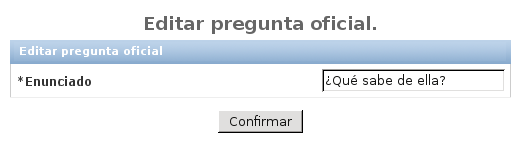
\includegraphics[scale=0.55]{4.Funcionamiento_Aplicacion/4.3.Gestion/4.3.1.Administrador_Principal/4.3.1.19.PreguntaOficial/edit_pregunta_oficial.png}
      }
      \caption{Captura de pantalla del formulario de edición de \textit{Pregunta oficial}.}
      \label{capturaEditPreguntaOficial}
    \end{center}
  \end{figure}

  \paragraph{}Una vez rellenado el formulario, se pulsará el botón
  \textit{Confirmar}, el cual se puede ver en la figura
  \ref{capturaBotonConfirmar}. Si el formulario rellenado es válido, y no tiene
  errores, se editará la información del elemento en el sistema. En caso de
  contener información no válida, un mensaje de error aparecerá indicando los
  campos del formulario que no han pasado la validación, los cuales habrá que
  modificar para modificar correctamente el elemento en el sistema.

